\begin{frame}{Le jeu de Go}
    \begin{block}{}
        \begin{columns}
            \begin{column}{8cm}
                \begin{itemize}
                    \item Le jeu de Go est un jeu de société chinois.
                    \item Joué sur une grille de 19x19 cases.
                    \item Deux joueurs, les blancs et les noirs.
                    \item Le but du jeu est de capturer le plus de territoires (pièces dans le tableau) et de prisonniers (pièces capturées) possibles.
                    \item Le jeu est très complexe, bien plus que les échecs, et il existe des milliers de stratégies différentes.
                \end{itemize}
            \end{column}
            \begin{column}{3cm}
                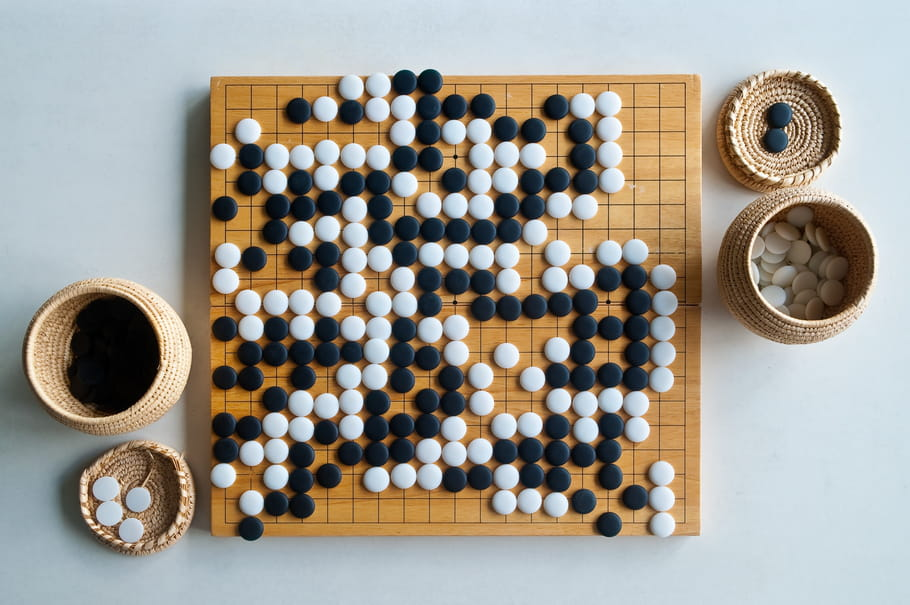
\includegraphics[width=3cm]{ressources/Go/Go_tableau}
            \end{column}
        \end{columns}
    \end{block}
\end{frame}


\begin{frame}{Le jeu de Go}{Analyse de complexité}
    \begin{block}{Echecs}
        \begin{itemize}
            \item Le nombre de positions légales est de l'ordre de $10^{46}$.
            \item Une approximation du nombre de parties possibles est de l'ordre de $10^{123}$.
        \end{itemize}
    \end{block}
    \pause
    \begin{alertblock}{Go}
        \begin{itemize}
            \item Le nombre de positions légales est de l'ordre de $10^{170}$.
            \item Une approximation du nombre de parties possibles entre des experts est de $10^{360}$.
        \end{itemize}
    \end{alertblock}
\end{frame}

\begin{frame}{Le jeu de Go}{Évolution des IA}
    \begin{block}{Chronologie}
        \begin{itemize}
            \item 1997: \textbf{Deep Blue} bat Kasparov, champion du monde d'échecs
            \item 2008: \textbf{MoGo} bat Catalin Taranu (5º dan professionnel) en 9x9
            \item 2013: \textbf{CrazyStone} bat Ishida Yoshio (9º dan professionnel) en 13x13 avec un handicap de 4 pierres
            \item 2016: \textbf{AlphaGo} bat Fan Hui (2º dan professionnel et champion d'Europe) sans handicap
            \item 2016: \textbf{AlphaGo} bat Lee Sedol (9º dan professionnel)
            \item 2017: \textbf{AlphaGo} bat Ke Jie (9º dan professionnel et numéro 1 mondial)
        \end{itemize}
    \end{block}
\end{frame}
